%
% loesung.tex -- Beispiel-File für die Beschreibung der Loesung
%
% (c) 2020 Prof Dr Andreas Müller, Hochschule Rapperswil
%
\section{Lösung
\label{quadratur:section:loesung}}
\subsection{Anwendung der Gauss-Legendre-Formel
\label{quadratur:subsection:gausslegendreanwendung}}
In dieser Subsektion versuchen wir, die Verwendung der Gauss-Legendre-Formel in einem
einfachen Beispiel herzuleiten, hierzu wird wieder die Funktion  
$I = \int_{-1}^{1}\sqrt{(1-x^2)}\,dx$ verwendet und 
wir berechnen die Formel mit vier Stützstellen.
\newline

\noindent
Zudem werden in der Tabelle~\ref{buch:table:gaussbeispielwerte} die Werte der 
Stützstellen und der Gewichte angegeben. Die Berechnung der Stützstellen, der Gewichte
und die verschiedenen Formen der Gauss-Quadratur werden in den folgenden Sektionen 
hergeleitet.

\begin{table}[h!]
    \centering
    \begin{tabular}{|c|c|}
        \hline
        Stützstellen $x_{i}$ & Gewichte $A_{i}$ \\
        \hline
        $-0.861136 $ & $ 0.347855 $ \\
        $-0.339981 $ & $ 0.652145 $ \\
        $ 0.339981 $ & $ 0.652145 $ \\
        $ 0.861136 $ & $ 0.347855 $ \\
        \hline
    \end{tabular}
    \caption{Werte für vier Stützstellen und deren Gewichte
    \label{buch:table:gaussbeispielwerte}}    
\end{table}

\noindent
In der Abbildung~\ref{quadratur:figure:gausslegendre1} sind die Vier Stützstellen 
ersichtlich.

\begin{figure}[!h]
    \centering
    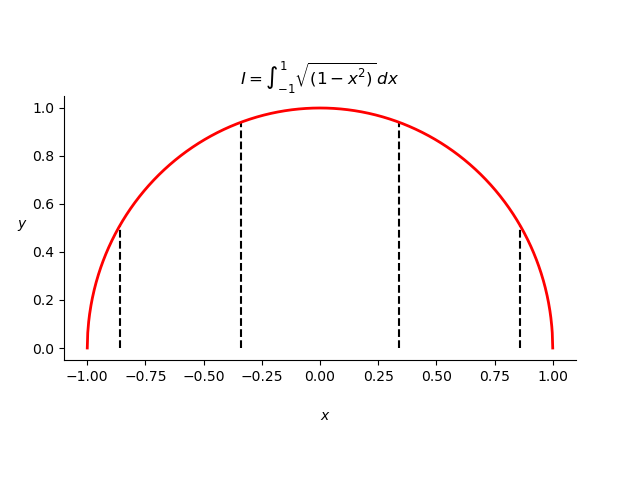
\includegraphics[scale=0.5]{papers/quadratur/figures/GaussLegendre1.png}
    \caption{
    \label{quadratur:figure:gausslegendre1}}
\end{figure}

\newpage
\noindent
Die Fläche unter dem Integral lässt sich nun mit der Formel 

\begin{equation}
    I 
    =
    \int_{-1}^{1} f(x) 
    \approx
    \sum_{i=0}^{n} A_{i} f(x_{i})
\end{equation}
\noindent 
berechnen, indem man die Stützstellen $x_{i}$ und die Gewichte $A_{i}$ einsetzt.

    \begin{align}
        I 
        &\approx 
        0.347855 \cdot \sqrt{1-(-0.861136)^{2}} 
        \notag
        \\
        &+ 
        0.652145 \cdot \sqrt{1-(-0.339981)^{2}} 
        \notag
        \\
        &+ 
        0.652145 \cdot \sqrt{1-(0.339981)^{2}} 
        \notag
        \\
        &+ 
        0.347855 \cdot \sqrt{1-(0.861136)^{2}} 
        \notag
        \\
        \notag
        \\
        &\approx 2 \cdot 0.652145 \cdot \sqrt{1-(0.339981)^{2}} + 2 \cdot 0.347855 \cdot \sqrt{1-(0.861136)^{2}} 
        \notag
        \\
        &\approx 1.226596 + 0.386863 
        \notag
        \\
        &\approx 1.580278
    \end{align}

\noindent
Das Resultat $1.580278$ ist bereits deutlich besser an der tatsächlichen Fläche $1.570796$ 
angenähert, als die Resultate der Trapezformel. 

\textcolor{red}{
    TODO
    \begin{itemize}
        \item Gauss Legendre Formel zeigen (Done)
        \item Beispiel berechnen mit Formel (Done)
        \item Berechnung der Gewichtung
        \item Berechnung der Position der Stützstellen
        \item Erklären der verschiedenen Formen der Gauss-Quadratur und ihrer Anwendungen
        \item 
    \end{itemize}
}


\subsection{De finibus bonorum et malorum
\label{quadratur:subsection:bonorum}}
\textcolor{red}{TODO: Lösung in python}


\subsection{Formen der Gauss-Quadratur
\label{quadratur:subsection:gaussformen}}
Es gibt verschiedene Ausprägungen der Gauss-Integration, abhängig vom jeweiligen Anwendungsbereich 
erkennbar an den Grenzen des Integrals und der Wahl der Gewichtung.
Die vier häufigsten Formen sind in der Tabelle~\ref{buch:table:gaussformen} abgebildet.

\begin{table}[h!]
    \begin{tabular}{|>{$}c<{$}|>{$}c<{$}|>{$}c<{$}|>{$}c<{$}|}
        \hline
        \text{Name} &  \text{Untere Grenze} & \text{Obere Grenze} & \text{Formel} \\
        \hline  
        \text{Legendre} & -1 & 1 & p_{n}(x) = \int_{-1}^{1} f(x)\,dx \approx \sum_{i=0}^{n} A_{i} f(x_{i}) \\
        \text{Chebyshev} &  -1 & 1 & T_{n}(x) = \int_{-1}^{1} (1-x^{2})^{-1/2} f(x)\,dy \approx \frac{\pi}{n+1} \sum_{i=0}^{n} f(x_{i}) \\
        \text{Laguerre} &  0 & \infty & L_{n}(x) = \int_{0}^{\infty} e^{-x} f(x)\,dx \approx \sum_{i=0}^{n} A_{i} f(x_{i}) \\
        \text{Hermite} & -\infty & \infty & H_{n}(x) = \int_{-\infty}^{\infty} f(x)\,dx \approx \sum_{i=0}^{n} A_{i} f(x_{i})\\
        \hline
    \end{tabular}
    \caption{Formen der Gauss-Quadratur
    \label{buch:table:gaussformen}}
    
\end{table}


